
\documentclass[12pt]{article}
\usepackage{amssymb,amsmath,graphicx,multicol}
\usepackage[margin=0.5in]{geometry}
\newcommand{\ds}{\displaystyle}

\setlength{\topmargin}{-.9in}
\setlength{\textwidth}{6.8in}
\setlength{\textheight}{9.5in}
\setlength{\oddsidemargin}{-.2in}
\setlength{\evensidemargin}{-.2in}

\setlength{\parindent}{0pt}
\pagestyle{empty}
\begin{document}
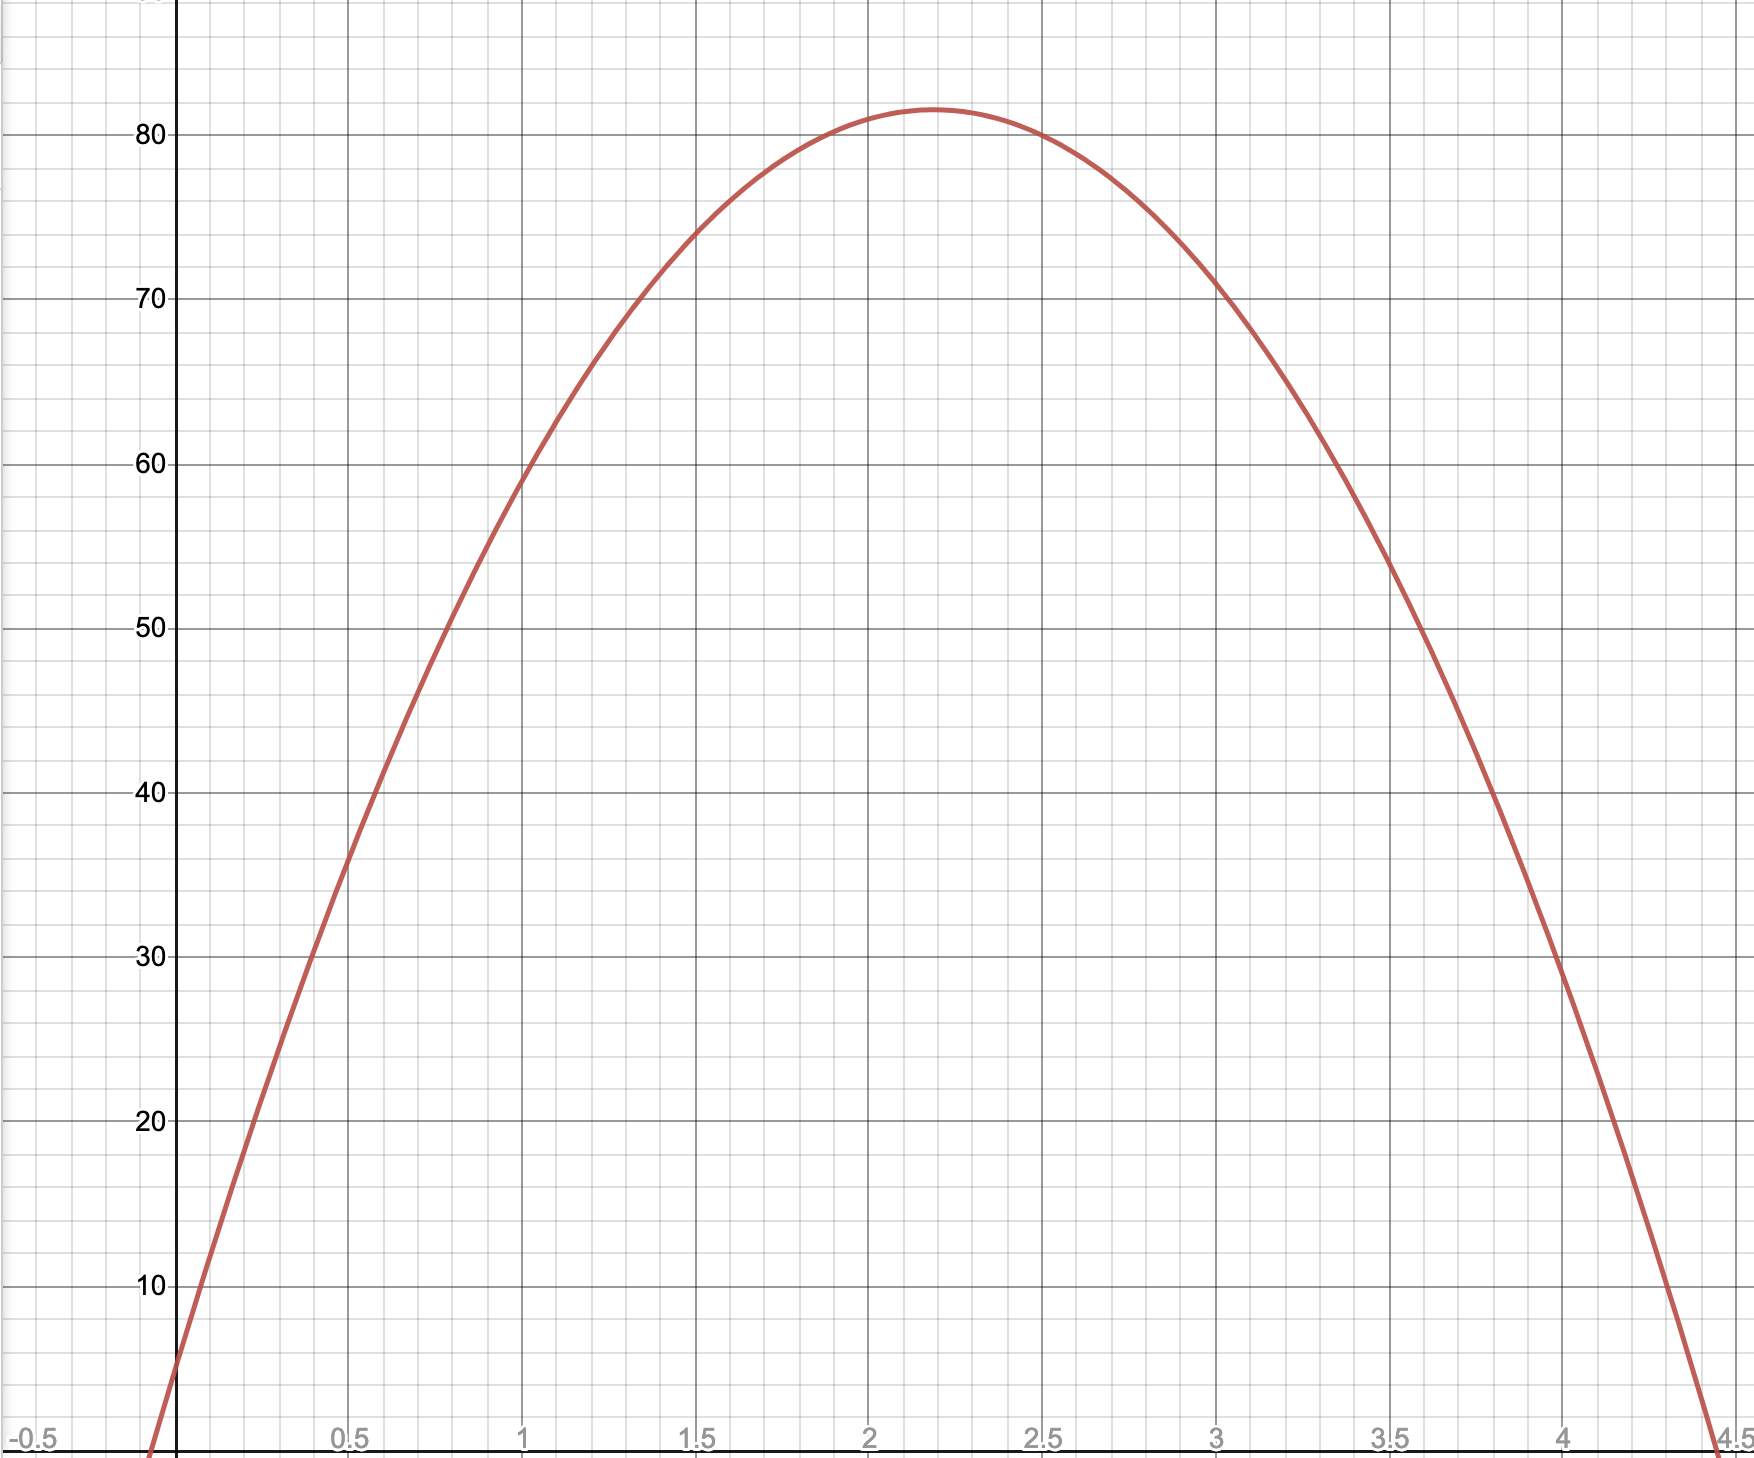
\includegraphics[scale=0.6]{spud2.png}\\ \\ \\ 
	\begin{tabular}{|r|ccccccccc|}
	\hline
	$t$ (time, s) & 0 & 0.5 & 1 & 1.5 & 2 & 2.5 & 3 & 3.5 & 4\\
	\hline
	$f(t)= y$ (height, ft) & 5 & 36 & 59 & 74 & 81 & 80 & 71 & 54 & 29\\
	\hline
	\end{tabular}
        \\
        \hspace{-0.5in}
        \begin{tabular}{rcccc}
          \hline
          \(t\)&\quad 0\quad&\quad 0.5\quad&\quad 1\quad&\quad 1.5\quad\\
          \hline
          Avg velocity from \(t\) to \(2\)&&&&\\
        \end{tabular}\\ \\ \\
        \begin{tabular}{rcccc}
          \hline
          \(t\)&\quad2.5\quad&\quad 3\quad&\quad3.5\quad &\quad 4\quad\\
          \hline
          Avg velocity from \(2\) to \(t\)
        \end{tabular}
        \\ \vspace{1in} \\ 
        \begin{tabular}{|r|ccccc|}
          \hline
          \(t\) &1.9&1.99&2&2.01&2.1\\
          \hline
          \(f(t)=y\)&80.24&80.9384&81&81.0584&81.44\\
          \hline
        \end{tabular}
\end{document}
%%% Local Variables:
%%% mode: latex
%%% TeX-master: t
%%% End:
